\begin{figure}[ht]
    \centering
    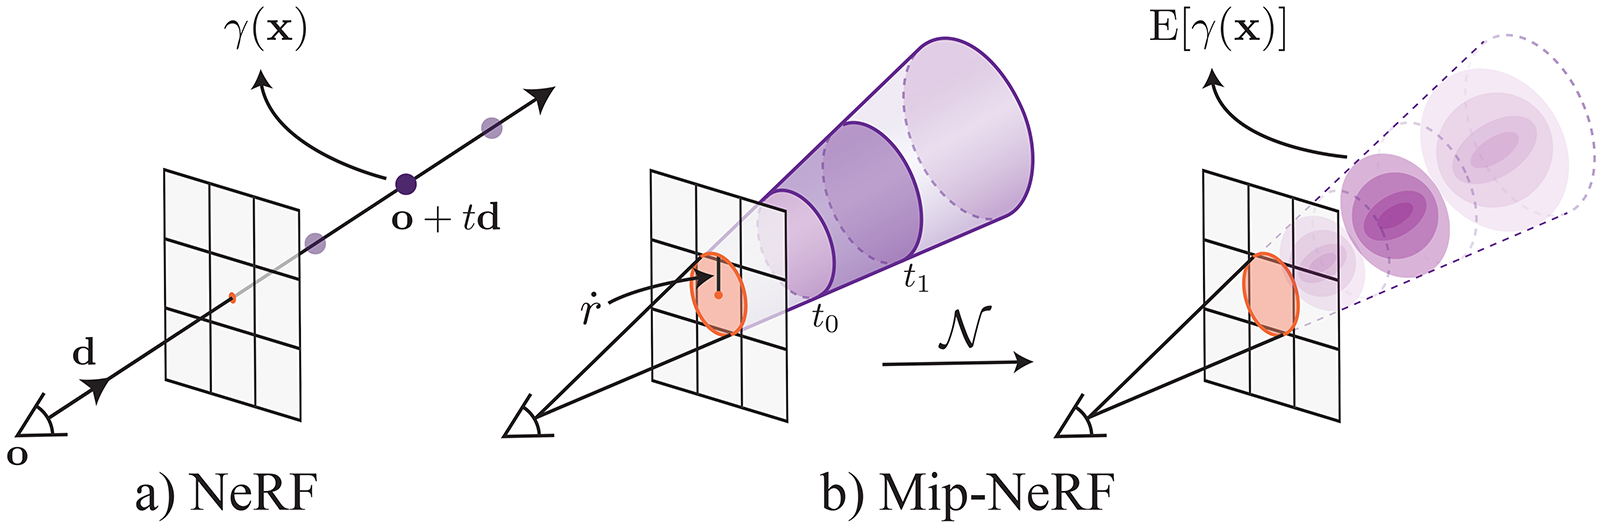
\includegraphics[width=1.0\textwidth]{figures/mip-nerf-frustums.png}
    \caption[Illustration of positional encoding]{A comparison of sampling strategies. NeRF (a) samples points along rays traced through each pixel before positionally encoding the points. Mip-NeRF (b) cast cones through the pixels' footprint and into the volume before applying \acrfull{ipe}. Figure 1 from Mip-NeRF \cite{barron_mip-nerf_2021}.}
    \label{fig:mip-nerf-frustums}
\end{figure}